\documentclass[11pt]{beamer}
\usepackage{listings} % Include the listings-package
\usepackage[T1]{fontenc}
\usepackage[utf8]{inputenc}
\usepackage[english]{babel}
\usepackage{amsmath}
\usepackage{amssymb, amsfonts, latexsym, cancel}
\usepackage{float}
\usepackage{graphicx}
\usepackage{epstopdf}
\usepackage{subfigure}
\usepackage{hyperref}
%\usepackage{authblk}
\usepackage{blindtext}
\usepackage{booktabs} % Allows the use of \toprule, 
\usepackage{filecontents}
\usepackage{courier} %% Sets font for listing as Courier.
\usepackage{listings}
%\usepackage{listings, xcolor}
\lstset{
tabsize = 2, %% set tab space width
showstringspaces = false, %% prevent space marking in strings, string is defined as the text that is generally printed directly to the console
numbers = left, %% display line numbers on the left
commentstyle = \color{green}, %% set comment color
keywordstyle = \color{blue}, %% set keyword color
stringstyle = \color{red}, %% set string color
rulecolor = \color{black}, %% set frame color to avoid being affected by text color
basicstyle = \small \ttfamily , %% set listing font and size
breaklines = true, %% enable line breaking
numberstyle = \tiny,
}
\usepackage{caption}
\DeclareCaptionFont{white}{\color{white}}
\DeclareCaptionFormat{listing}{\colorbox{gray}{\parbox{\textwidth}{#1#2#3}}}
\captionsetup[lstlisting]{format=listing,labelfont=white,textfont=white}
\definecolor{urlColor}{rgb}{0.06, 0.3, 0.57}
\definecolor{linkColor}{rgb}{0.57, 0.0, 0.04}
\definecolor{fileColor}{rgb}{0.0, 0.26, 0.26}
\hypersetup{
    colorlinks=true,
    linkcolor=linkColor,
    filecolor=fileColor,      
    urlcolor=urlColor,
}
\urlstyle{same}
\setbeamercovered{transparent}
%\usetheme{Boadilla}
\usetheme{CambridgeUS}
%\usetheme{Berkeley}
%\usetheme{Warsaw}
%\usetheme{Madrid}

\title[Interfaz de usuario]{\bf\Huge Nielsen y Molich}
\subtitle{}

\author[Grupo 12]
{
	Anampa Chura Diego David \\
	Flores Quispe Percy Santiago \\
	Mamani Condori Kevin Alonso \\
	Paniura Huamani Jose Maykol  
}
\institute[UNSA]
{
\inst{1}% 
System Engineering School\\
System Engineering and Informatic Department\\
Production and Services Faculty\\
San Agustin National University of Arequipa
}

\date[2020-09-15]{\scriptsize{2020-09-16}}
%\logo{
\includegraphics[width=3.0cm]{img/logo_unsa.jpg}}
\titlegraphic{
\includegraphics[width=2.0cm]{img/logo_unsa.jpg}}

\begin{document}

\begin{frame}
\titlepage
\end{frame}

\begin{frame}
\frametitle{Contenido}
\tableofcontents
\end{frame}

\section{Nielsen y Molich}
%References frame
\begin{frame}
\frametitle{Nielsen y Molich}
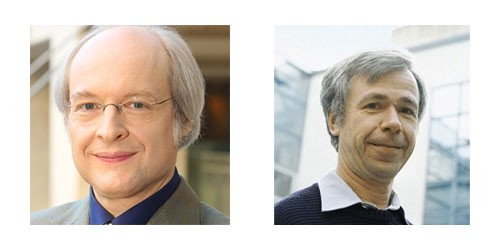
\includegraphics[width=6.0cm,height=4.0cm]{img/NielsenMolich.jpeg}\centering

\begin{itemize}
\item Nielsen y Molich (1990) ofrecieron un conjunto de reglas de diseño para su uso en la evaluación heurística de interfaces de usuario
\item Improving a human-computer dialogue (Book)
\item 10 Principios Heurísticos de Nielsen
\item Evaluación Heurística (EH), permite examinar la calidad de uso de una interfaz por parte de varios evaluadores expertos
\end{itemize}
\end{frame}

\section{1.-Visibilidad del estado del sistema:}
%References frame
\begin{frame}
\frametitle{1.-Visibilidad del estado del sistema:}

\begin{itemize}
\item El usuario debe estar informado de las operaciones del sistema, estás operaciones deben ser altamente visible y que se muestre en pantalla dentro de un periodo de tiempo razonable de manera que para el usuario sea fácil de entender
\item \bf Buena Practica:\\ En la web de Vueling el usuario sabe en todo momento el estado del sistema. Se le informa qué información ha buscado previamente y en qué página del proceso de compra se encuentra
\end{itemize}

\begin{figure}
  \centering
  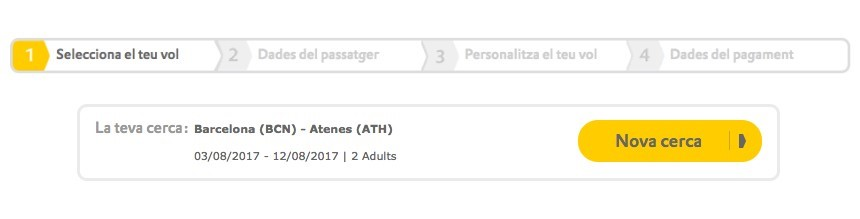
\includegraphics[width=8.0cm,height=2.0cm]{img/Imagen1.jpg}
\end{figure}
\end{frame}

\section{2.-Empate entre el sistema y el mundo real:}
%References frame
\begin{frame}
\frametitle{2.-Empate entre el sistema y el mundo real:}

\begin{itemize}
\item El sistema debe hablar en el lenguaje del usuario, con palabras, frases y conceptos familiares para él. Utilizar convenciones del mundo real, haciendo que la información aparezca en un orden natural y lógico
\item Buena Practica:\\  Airbnb en su buscador principal
\end{itemize}

\begin{figure}
  \centering
  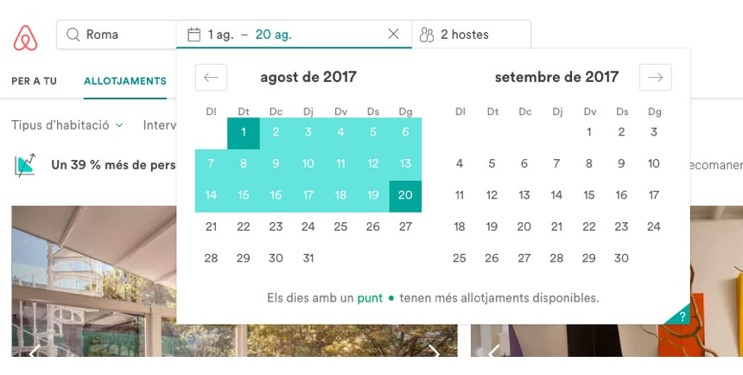
\includegraphics[width=8.0cm,height=4.0cm]{img/Imagen2.jpg}
\end{figure}
\end{frame}

\section{3.-Control y libertad del usuario:}
%References frame
\begin{frame}
\frametitle{3.-Control y libertad del usuario:}

\begin{itemize}
\item El usuario debe tener la opción de hacer pasos hacia atrás en cualquier proceso y que sean posibles incluyendo rehacer y deshacer acciones anteriores ya que a menudo los usuarios eligen funcionalidades por error y necesitan salir del estado indeseado
\item Buena Practica:\\ Gmail permite deshacer la acción de envío de correos electrónicos
\end{itemize}

\begin{figure}
  \centering
  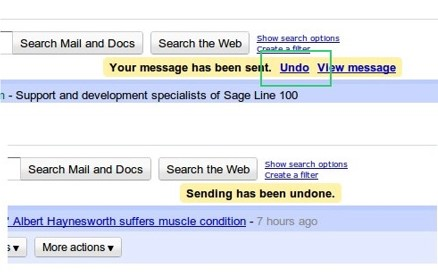
\includegraphics[width=8.0cm,height=4.0cm]{img/Imagen3.jpg}
\end{figure}
\end{frame}

\section{4.-Consistencia y estándares:}
%References frame
\begin{frame}
\frametitle{4.-Consistencia y estándares:}

\begin{itemize}
\item El diseñador de la interfaz debe asegurar que los elementos gráficos y su terminología se mantenga en todas las pantallas o plataformas similares. Que se sigan las normas y convenciones de la plataforma sobre la que está implementando el sistema
\end{itemize}

\begin{figure}
  \centering
  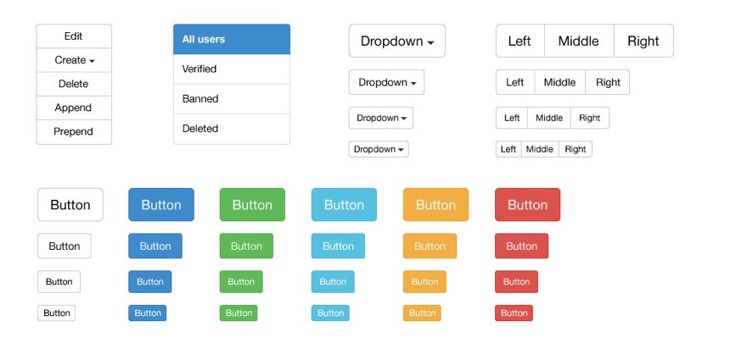
\includegraphics[width=8.0cm,height=4.0cm]{img/Imagen4.jpg}
\end{figure}
\end{frame}

\section{5.-Prevención de errores:}
%References frame
\begin{frame}
\frametitle{5.-Prevención de errores:}

\begin{itemize}
\item Los sistemas deben ser capaces de que los errores potenciales se mantengan al mínimo; de tal forma, que el usuario no debe detectar y solucionar problemas sino al contrario, el sistema le debe ofrecer posibles soluciones
\item Buena Practica:\\ El formulario en el
proceso de ‘Registro’ de Facebook
\end{itemize}

\begin{figure}
  \centering
  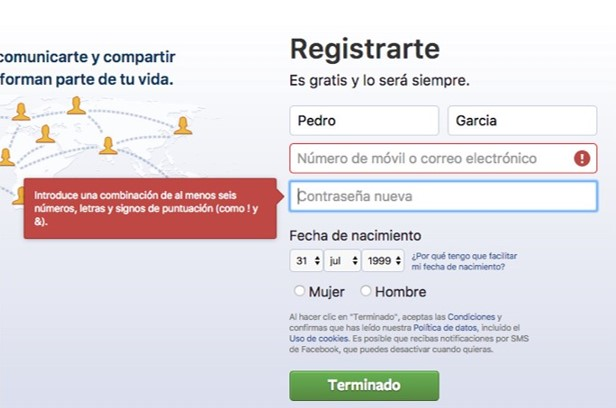
\includegraphics[width=8.0cm,height=4.0cm]{img/Imagen5.jpg}
\end{figure}
\end{frame}

\section{6.-Reconocimiento mejor que recuerdo:}
%References frame
\begin{frame}
\frametitle{6.-Reconocimiento mejor que recuerdo:}

\begin{itemize}
\item Crear interfaces que hagan que los objetos, acciones, opciones y direcciones sean visibles y fácilmente reconocibles para el usuario, es decir, el usuario no debería tener que recordar la información de una parte del diálogo a otra
\item Buena Practica:\\ Página web de Atrápalo se muestra una leyenda que muestra los parámetros utilizados
\end{itemize}

\begin{figure}
  \centering
  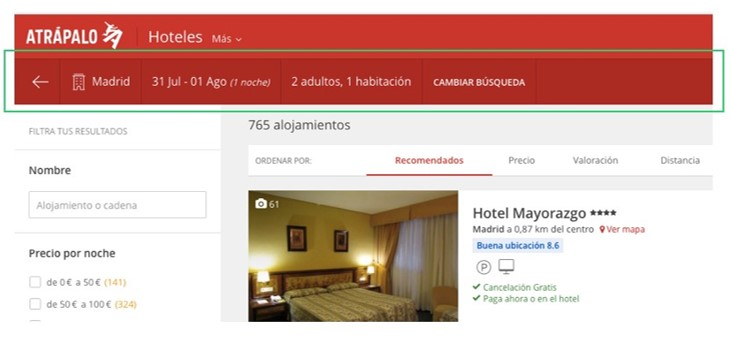
\includegraphics[width=8.0cm,height=4.0cm]{img/Imagen6.jpg}
\end{figure}
\end{frame}

\section{7.-Flexibilidad y eficiencia de uso:}
%References frame
\begin{frame}
\frametitle{7.-Flexibilidad y eficiencia de uso:}

\begin{itemize}
\item Al mayor uso de un sistema viene la demanda de menos interacciones que permitan una navegación más rápida; de este manera, el sistema debe servir para usuarios inexpertos y experimentados
\item Buena Practica:\\ Twitter proporciona atajos de teclado que mejoran la interacción de los usuarios expertos
\end{itemize}

\begin{figure}
  \centering
  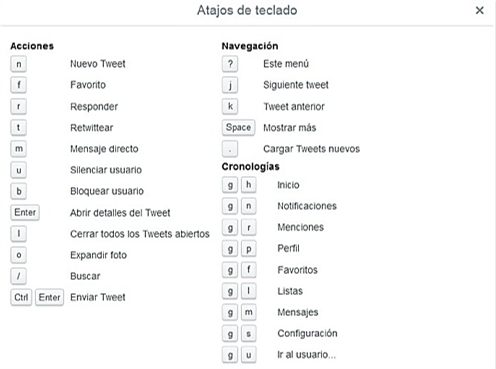
\includegraphics[width=8.0cm,height=4.0cm]{img/Imagen7.png}
\end{figure}
\end{frame}

\section{8.-Diseño estético y minimalista:}
%References frame
\begin{frame}
\frametitle{8.-Diseño estético y minimalista:}

\begin{itemize}
\item Los diálogos no deberían contener información irrelevante o que se necesite raramente ya que la información innecesaria puede distraer al usuario y disminuir la visibilidad relativa
\item Buena Practica:\\ Google no añade información innecesaria en su página inicial; dando así protagonismo a su funcionalidad principal: el buscador
\end{itemize}

\begin{figure}
  \centering
  
\includegraphics[width=8.0cm,height=4.0cm]{img/Imagen8.jpg}
\end{figure}
\end{frame}

\section{9.-Ayudar a reconocer, diagnosticar y recuperarse de errores:}
%References frame
\begin{frame}
\frametitle{9.-Ayudar a reconocer, diagnosticar y recuperarse de errores:}

\begin{itemize}
\item Los mensajes de error deben estar expresados en lenguaje llano (sin códigos), indicando con precisión el problema y sugiriendo una solución
\item Buena Practica:\\ La página de error 404 en la web oficial de Spotify; dónde se informa sobre el problema y posibles salidas para solucionarlo
\end{itemize}

\begin{figure}
  \centering
  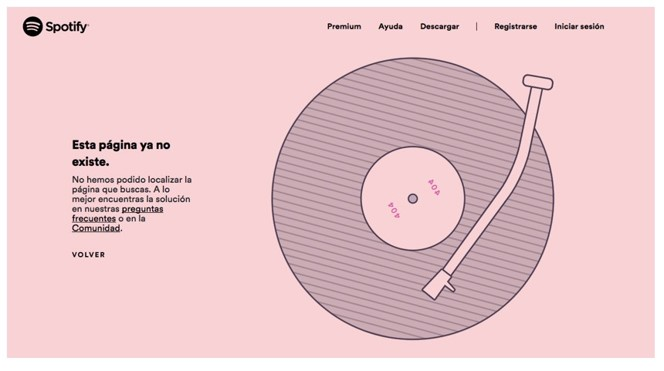
\includegraphics[width=8.0cm,height=4.0cm]{img/Imagen9.jpg}
\end{figure}
\end{frame}

\section{10.-Ayuda y documentación:}
%References frame
\begin{frame}
\frametitle{10.-Ayuda y documentación:}

\begin{itemize}
\item Es necesario proveer al usuario de ayuda y documentación, los cuales deben ser fácil de buscar, centrada en la tareas del usuario, con información de las etapas a realizar y que no sea muy extensa
\item Buena Practica:\\ Portal Stackoverflow proporciona una detallada sección de ayuda en su ‘Help center’
\end{itemize}

\begin{figure}
  \centering
  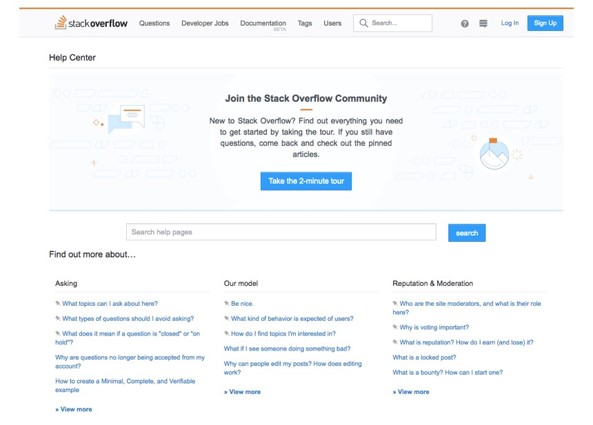
\includegraphics[width=8.0cm,height=4.0cm]{img/Imagen10.jpg}
\end{figure}
\end{frame}


\section{Referencias:}
%References frame
\begin{frame}
\frametitle{Referencias:}
\begin{itemize}
\item Nielsen, J., & Molich, R. (1990, March). Heuristic evaluation of user interfaces. In Proceedings of the SIGCHI conference on Human factors in computing systems (pp. 249-256)
\item Xiii, Jhonson J. (2014). Designing with the Mind in mind 2nd. Edition
\item Biografia Metodologías de UX: \url{https://blog.interactius.com/metodologías-de-ux-evaluación-heurística-parte-i-b5d02b566987/}
\item Biografia Reglas heurísticas: \url{https://www.uifrommars.com/10-reglas-heuristicas-como-aplicarlas/}
\end{itemize}
\end{frame}

\end{document}